\setlength{\parindent}{25pt}
\setlength{\parskip}{0em}
\fontsize{11}{14}\selectfont

\clearpage

\appendix
\section{Chilean yellow lobster squat stock assessment} \label{app:model}
\subsection{Population Dynamics}

The annual survivorship as well as the equilibrium 
yield under a given fishing mortality rate $F_{t,\tau}$, were modelled 
using the equations
\[ 
N_{t,a}=\begin{cases} N_{t,r}, & a=1\\
N_{t-1,a-1}e^{-Z_{t-1,a-1}},& a>1\\
N_{t-1,a-1}e^{-Z_{t-1,a-1}} + N_{t-1,a}e^{-Z_{t-1,a}},& a=A^+,
\end{cases}  
\]
where $N_{t,r}$ represent the annual recruitment for year $t$ 
assuming a Beverton-Holt stock-recruitment relationship,  
$N_{t,a}$ is the number of individual 
of age $a$ a at the start of year $t$, $A^+$ is the plus group for age, and $e^{-Z_{t,a}}$ represent
the survivorship fraction after annual harvest. 
Total annual mortality rate,
\[ 
Z_{t,a}= M+\left( F_{t,\tau}\psi_{a}\right), 
\]
integrates the instantaneous 
natural mortality rate $M$, together with both the fishing mortality $F_{t,\tau}$
derived from the $\tau$-\textit{th} HCR and the age-specific 
fishing selectivity $\psi_a$. The gear-selection fishing follow a dome-shape age-based curve given by:
\[ 
\psi_{a}=\begin{cases}e^{-(a-\gamma)^2 / \sigma^{2}_l}, & a\leq \gamma\\
e^{-(a-\gamma)^2 / \sigma^{2}_r}, & a > \gamma
\end{cases}  
\]
where $\gamma$ is the age of full selectivity, and $\sigma_l$ and 
$\sigma_r$ represents the left and right side standard deviations 
of a double half-gaussian function around $\gamma$, respectively. We used the dome-shape curve implemented in the most recent stock assessments, as many fishing operations are aimed to catch intermediates ages to maximise the catch rate, as well as  older fish are less susceptible after mid-season given the fleet displacement behaviour.

\clearpage

\section{Tables}

\begin{table}[ht]
\centering
\caption{Scenarios of mean length-at-entry age (L1) and the variation of the length at age (VLA) \vspace{0.5cm}}
\label{table1}
\begin{tabular}{c|c|c} \hline
\rowcolor[HTML]{EFEFEF} 
\textbf{Scenarios} & \textbf{L1} & \textbf{VLA} \\ \hline
1                  & -10\%       & -10\%        \\
2                  & Base        & -10\%        \\
3                  & +10\%       & -10\%        \\
4                  & -10\%       & Base         \\
5                  & Base        & Base         \\
6                  & +10\%       & Base         \\
7                  & -10\%       & +10\%        \\
8                  & Base        & +10\%        \\
9                  & +10\%       & +10\%       \\ \hline
\end{tabular}
\end{table}


\begin{table}[h]
\centering
\caption{Combinations of the steepness ($h$) values and recruitment variance (VAR) for each of nine (9) scenarios of L1 and VLA \vspace{0.5cm}}
\label{table2}
\begin{tabular}{c|c|c|c} \hline
\rowcolor[HTML]{EFEFEF} 
              & \textbf{$h$}    & \textbf{$\sigma^2_R$} & \textbf{N$^o$ scenarios} \\ \hline
Combination 1 & 1.0  & 0.2    & 9           \\
Combination 2 & 1.0  & 0.6    & 9           \\
Combination 3 & 1.0  & 1.0    & 9           \\
Combination 4 & 0.75 & 0.2    & 9           \\
Combination 6 & 0.75 & 0.6    & 9           \\
Combination 7 & 0.75 & 1.0    & 9          \\ \hline
\end{tabular}
\end{table}


\begin{table}[ht]
\centering
\caption{Simulation scenarios to explore the predictability of the growth parameters L1 and VLA and  productivity (h) with the assumption of a $\sigma^2_R=0.6$ \vspace{0.5cm}}
\label{table3}
\begin{tabular}{c|c|c|c|c|c|c|c} \hline
             & \multicolumn{3}{c|}{Simulator} &            & \multicolumn{3}{c}{Estimator}     \\ \hline
             & LMA      & VLA      & $h$       &            & LMA       & VLA       & $h$         \\ \hline
\rowcolor[HTML]{EFEFEF} 
Simulation 1 & -10\%    & Base     & 1.0     & scenario 1 & Estimated & Estimated & Estimated \\
\rowcolor[HTML]{EFEFEF} 
             & -10\%    & Base     & 1.0     & scenario 2 & Estimated & Estimated & Fixed     \\
Simulation 2 & +10\%    & Base     & 0.75    & scenario 3 & Estimated & Fixed     & Fixed     \\
             & +10\%    & +10\%    & 0.75    & scenario 4 & Fixed     & Estimated & Fixed    \\ \hline
\end{tabular}
\end{table}

\begin{table}[h]
\centering
\caption{Values of median relative bias (MSR) ad variation coefficient (CV) for all simulation scenarios. All simulations were run with a recruitment variance of $\sigma^2_R=0.6$. The percentage of convergence in each estimation scenarios \vspace{0.5cm}}
\label{table4}
\begin{tabular}{c|c|c|c|c|c|c|c} \hline
           & \multicolumn{2}{c|}{LMA} & \multicolumn{2}{c|}{VLA} & \multicolumn{2}{c|}{$h$} & Convergence \\ \hline
\rowcolor[HTML]{EFEFEF} 
           & MSR         & CV        & MSR        & CV         & MSR        & CV         & \%          \\ \hline
Scenario 1 & 0.11        & 0.04      & 0.07       & 0.02       & 0.14       & 0.11       & 46          \\
Scenario 1 & 0.99        & 0.04      & 0.03       & 0.02       & ---         & ---         & 100         \\
Scenario 1 & -0.12       & 0.09      & ---         & ---         & ---         & ---         & 100         \\
Scenario 1 & ---          & ---        & 0.05       & 0.03       & ---         & ---         & 94         \\ \hline
\end{tabular}
\end{table}


\clearpage
\section{Figures}


\begin{figure}[ht]
	\begin{center}
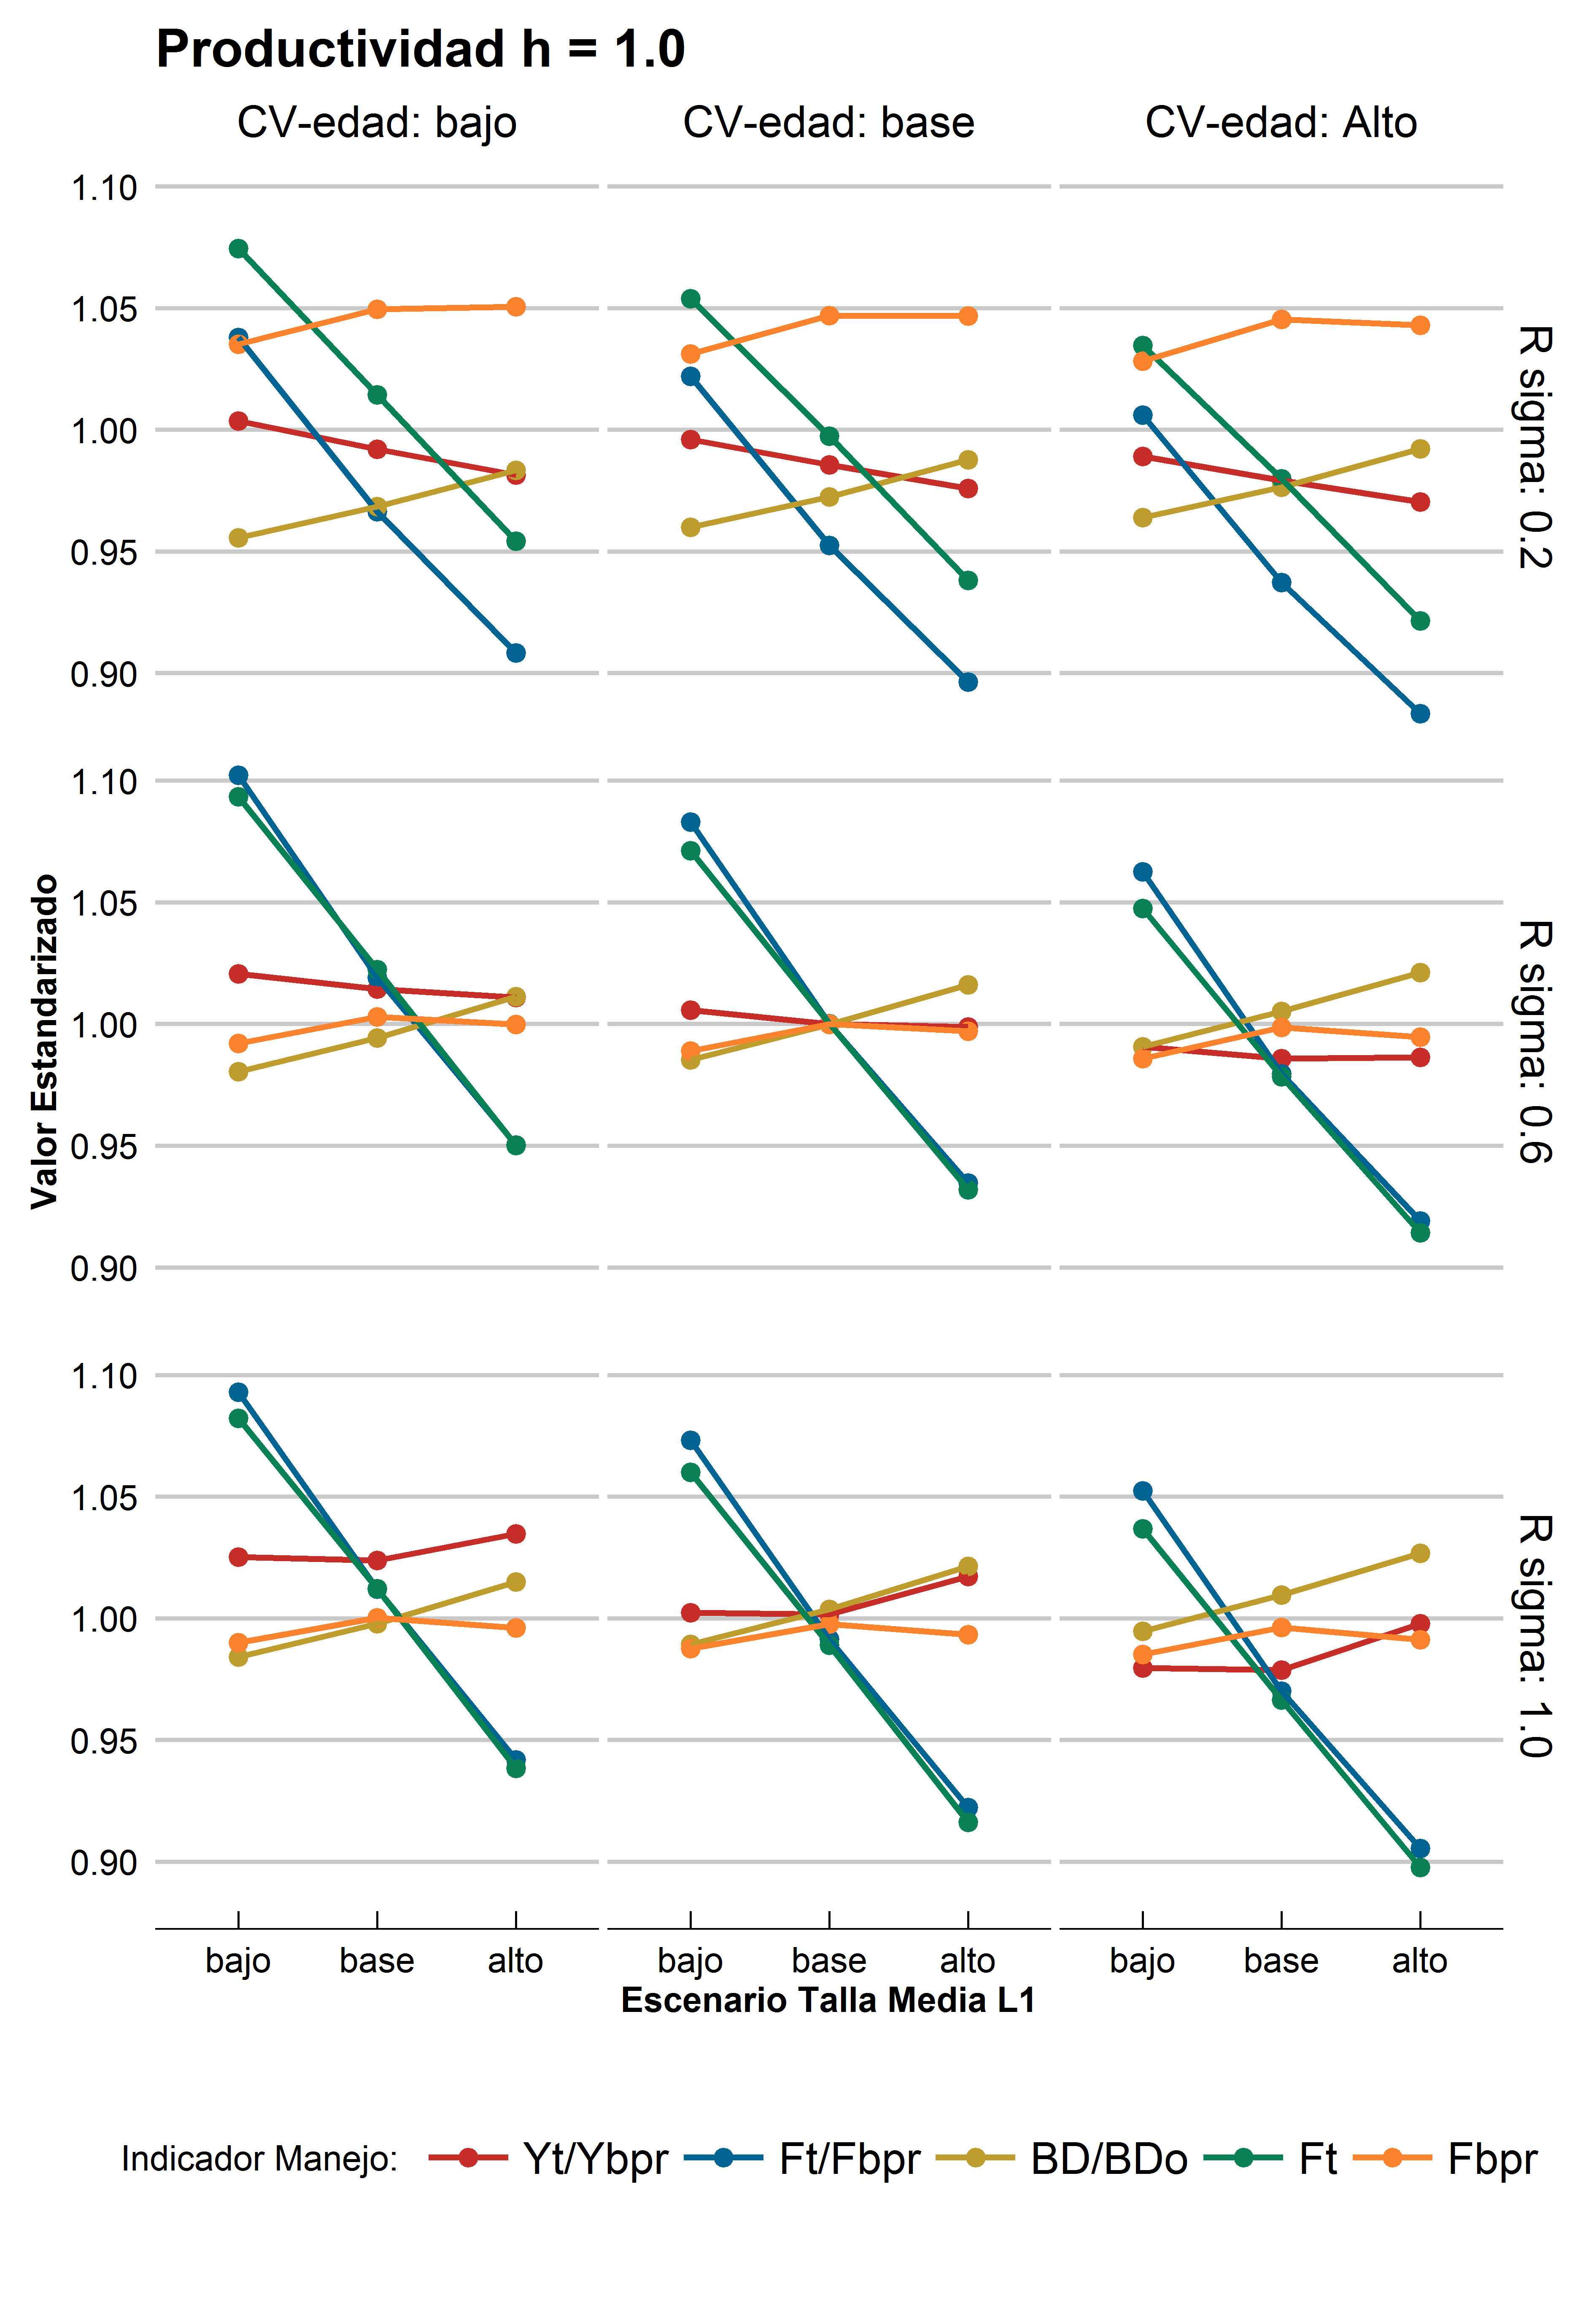
\includegraphics[width=0.70\columnwidth]{figures/steepness-10-var.png}
  \end{center}
\caption{Management advice indicators for scenario with productivity h=1.0. Contained the results of nine (9) scenarios of growth, (x-axis: mean length at-age L1) low (-10\%), Base, high (+10\%). Each column correspond to scenario of VLA, low (-10\%), Base, high (+10\%). Each row correspond to a recruitment variance value.}
\label{figure1}
\end{figure}


\begin{figure}[hbtp]
	\begin{center}
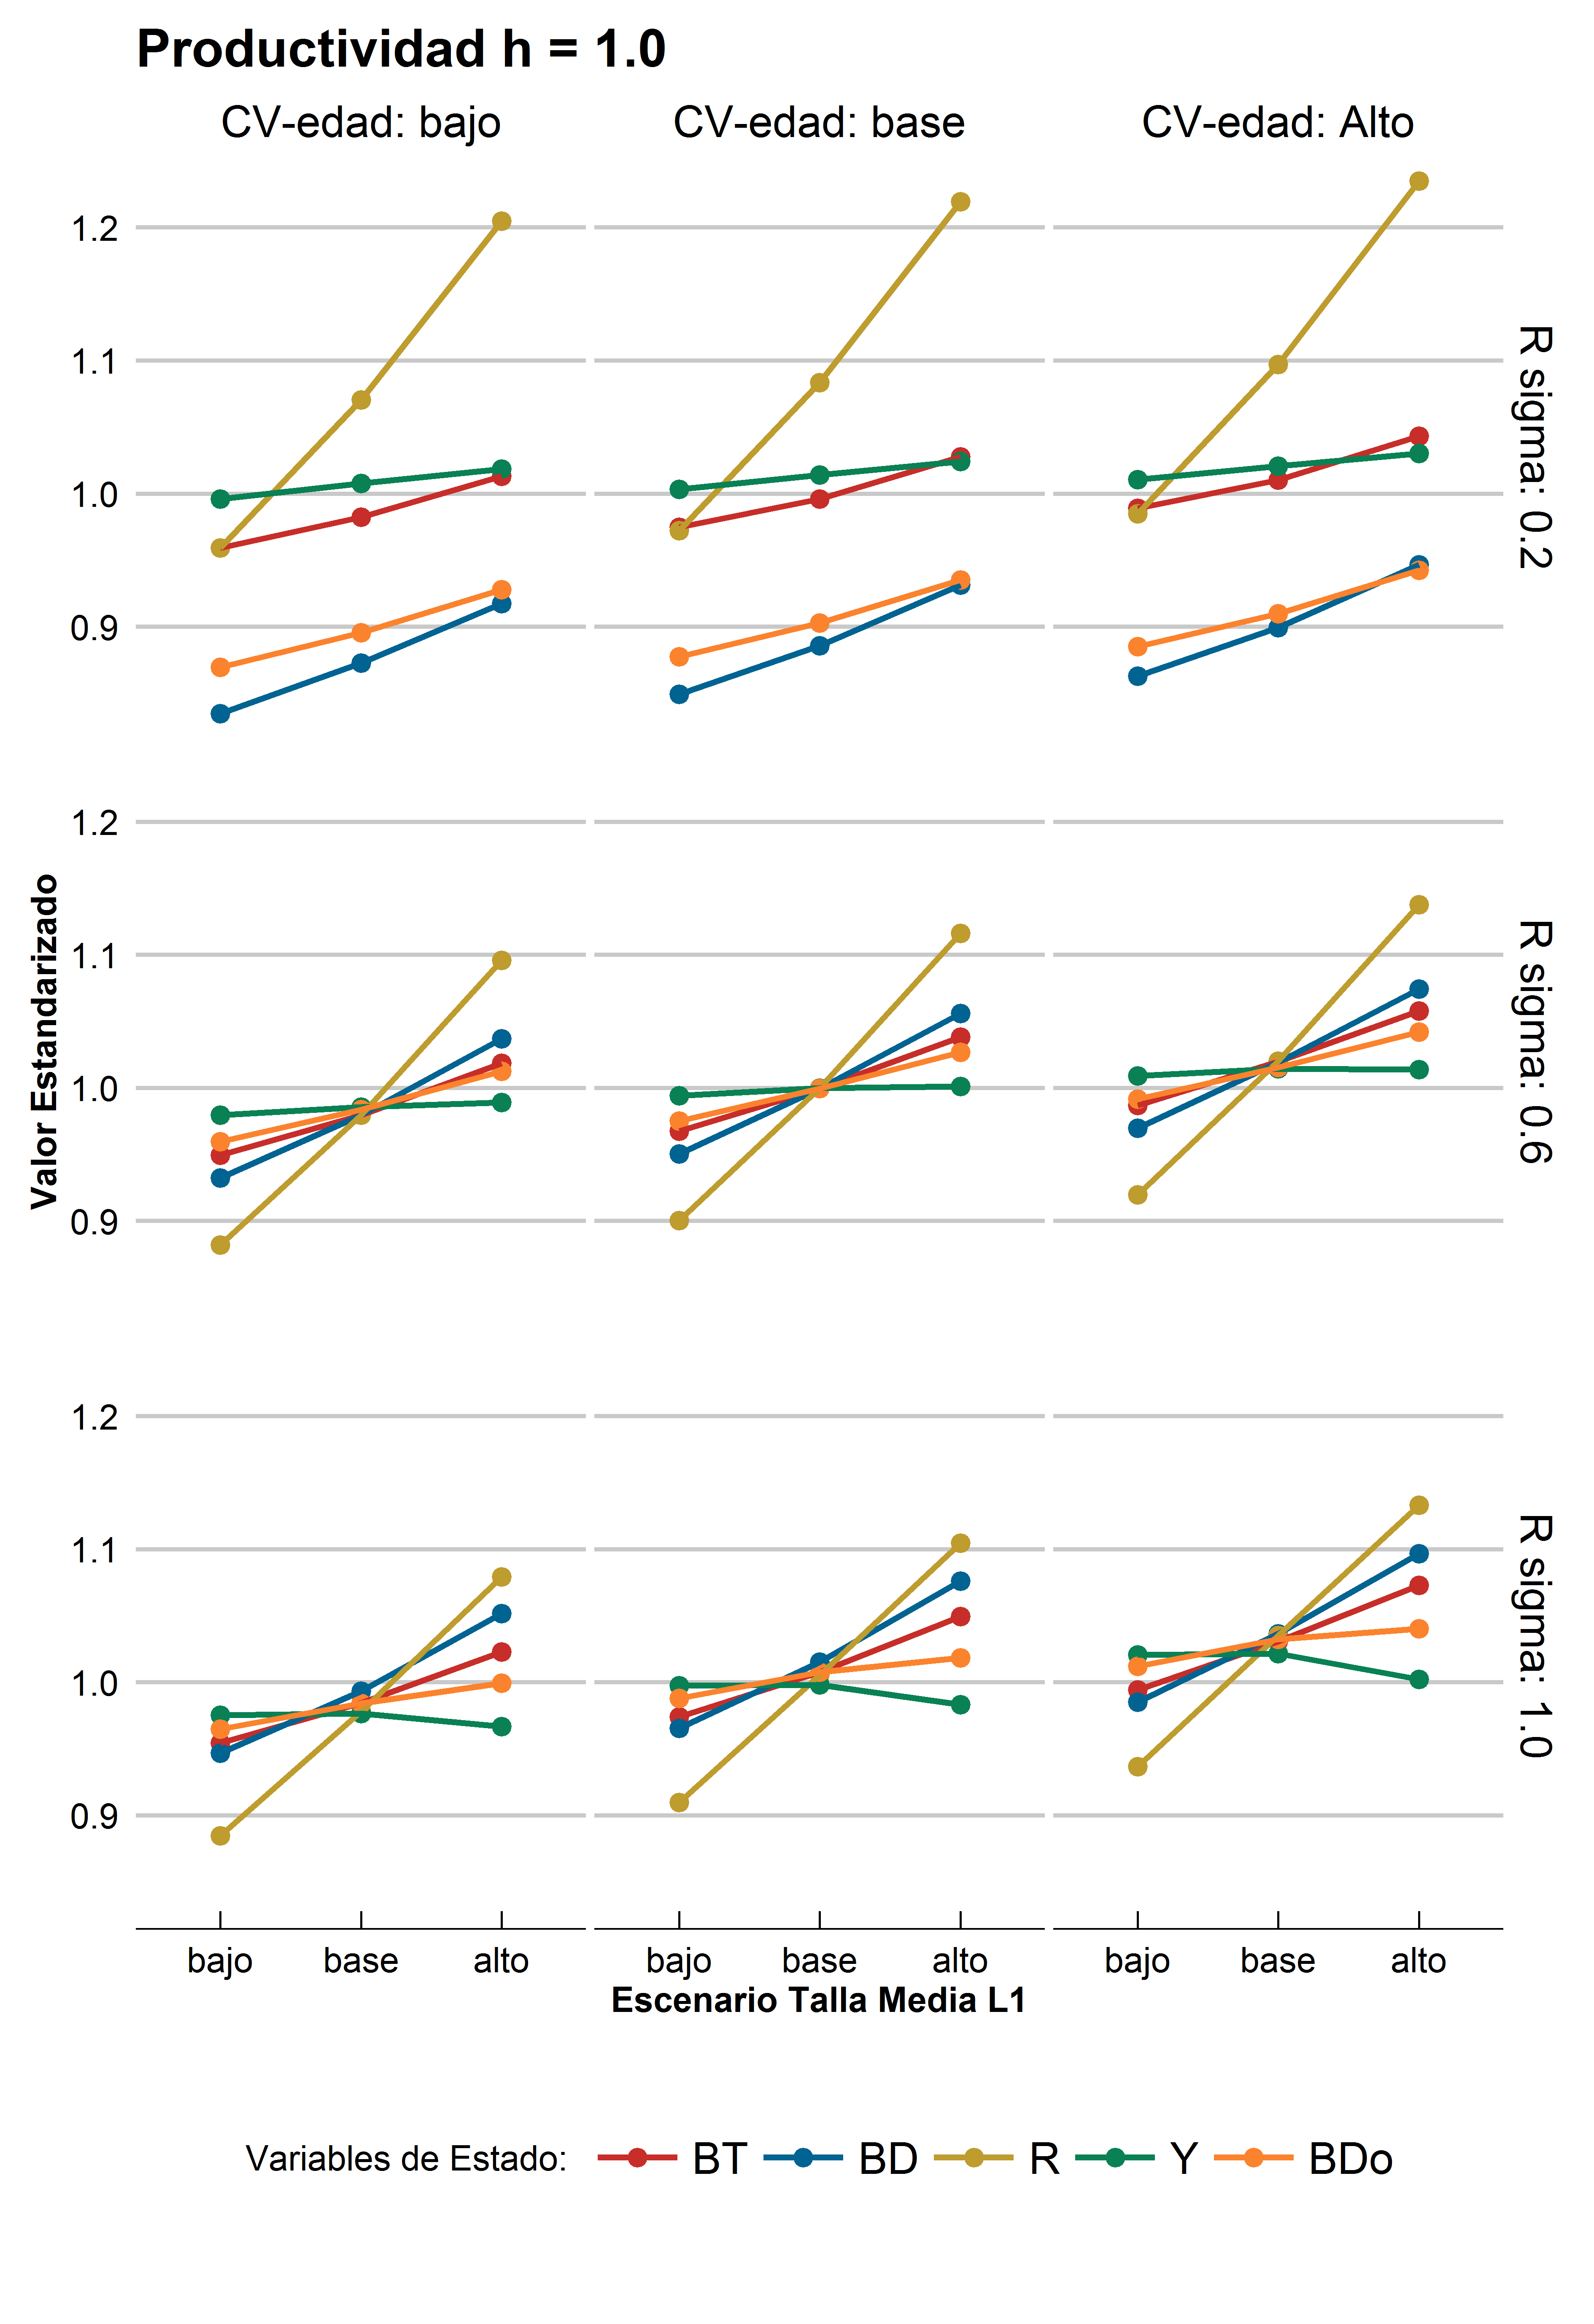
\includegraphics[width=0.70\columnwidth]{figures/steepness-10-estado.png}
  \end{center}
\caption{Stock assessment variables for scenario with productivity h=1.0. Contained the results of nine (9) scenarios of growth, (x-axis: mean length at-age L1) low (-10\%), Base, high (+10\%). Each column correspond to scenario of VLA, low (-10\%), Base, high (+10\%). Each row correspond to a recruitment variance value. Dashed black rectangle indicates the Base Case and should be equal to h=1. TODO---include rectangle}
\label{figure1}
\end{figure}


\begin{figure}[hbtp]
	\begin{center}
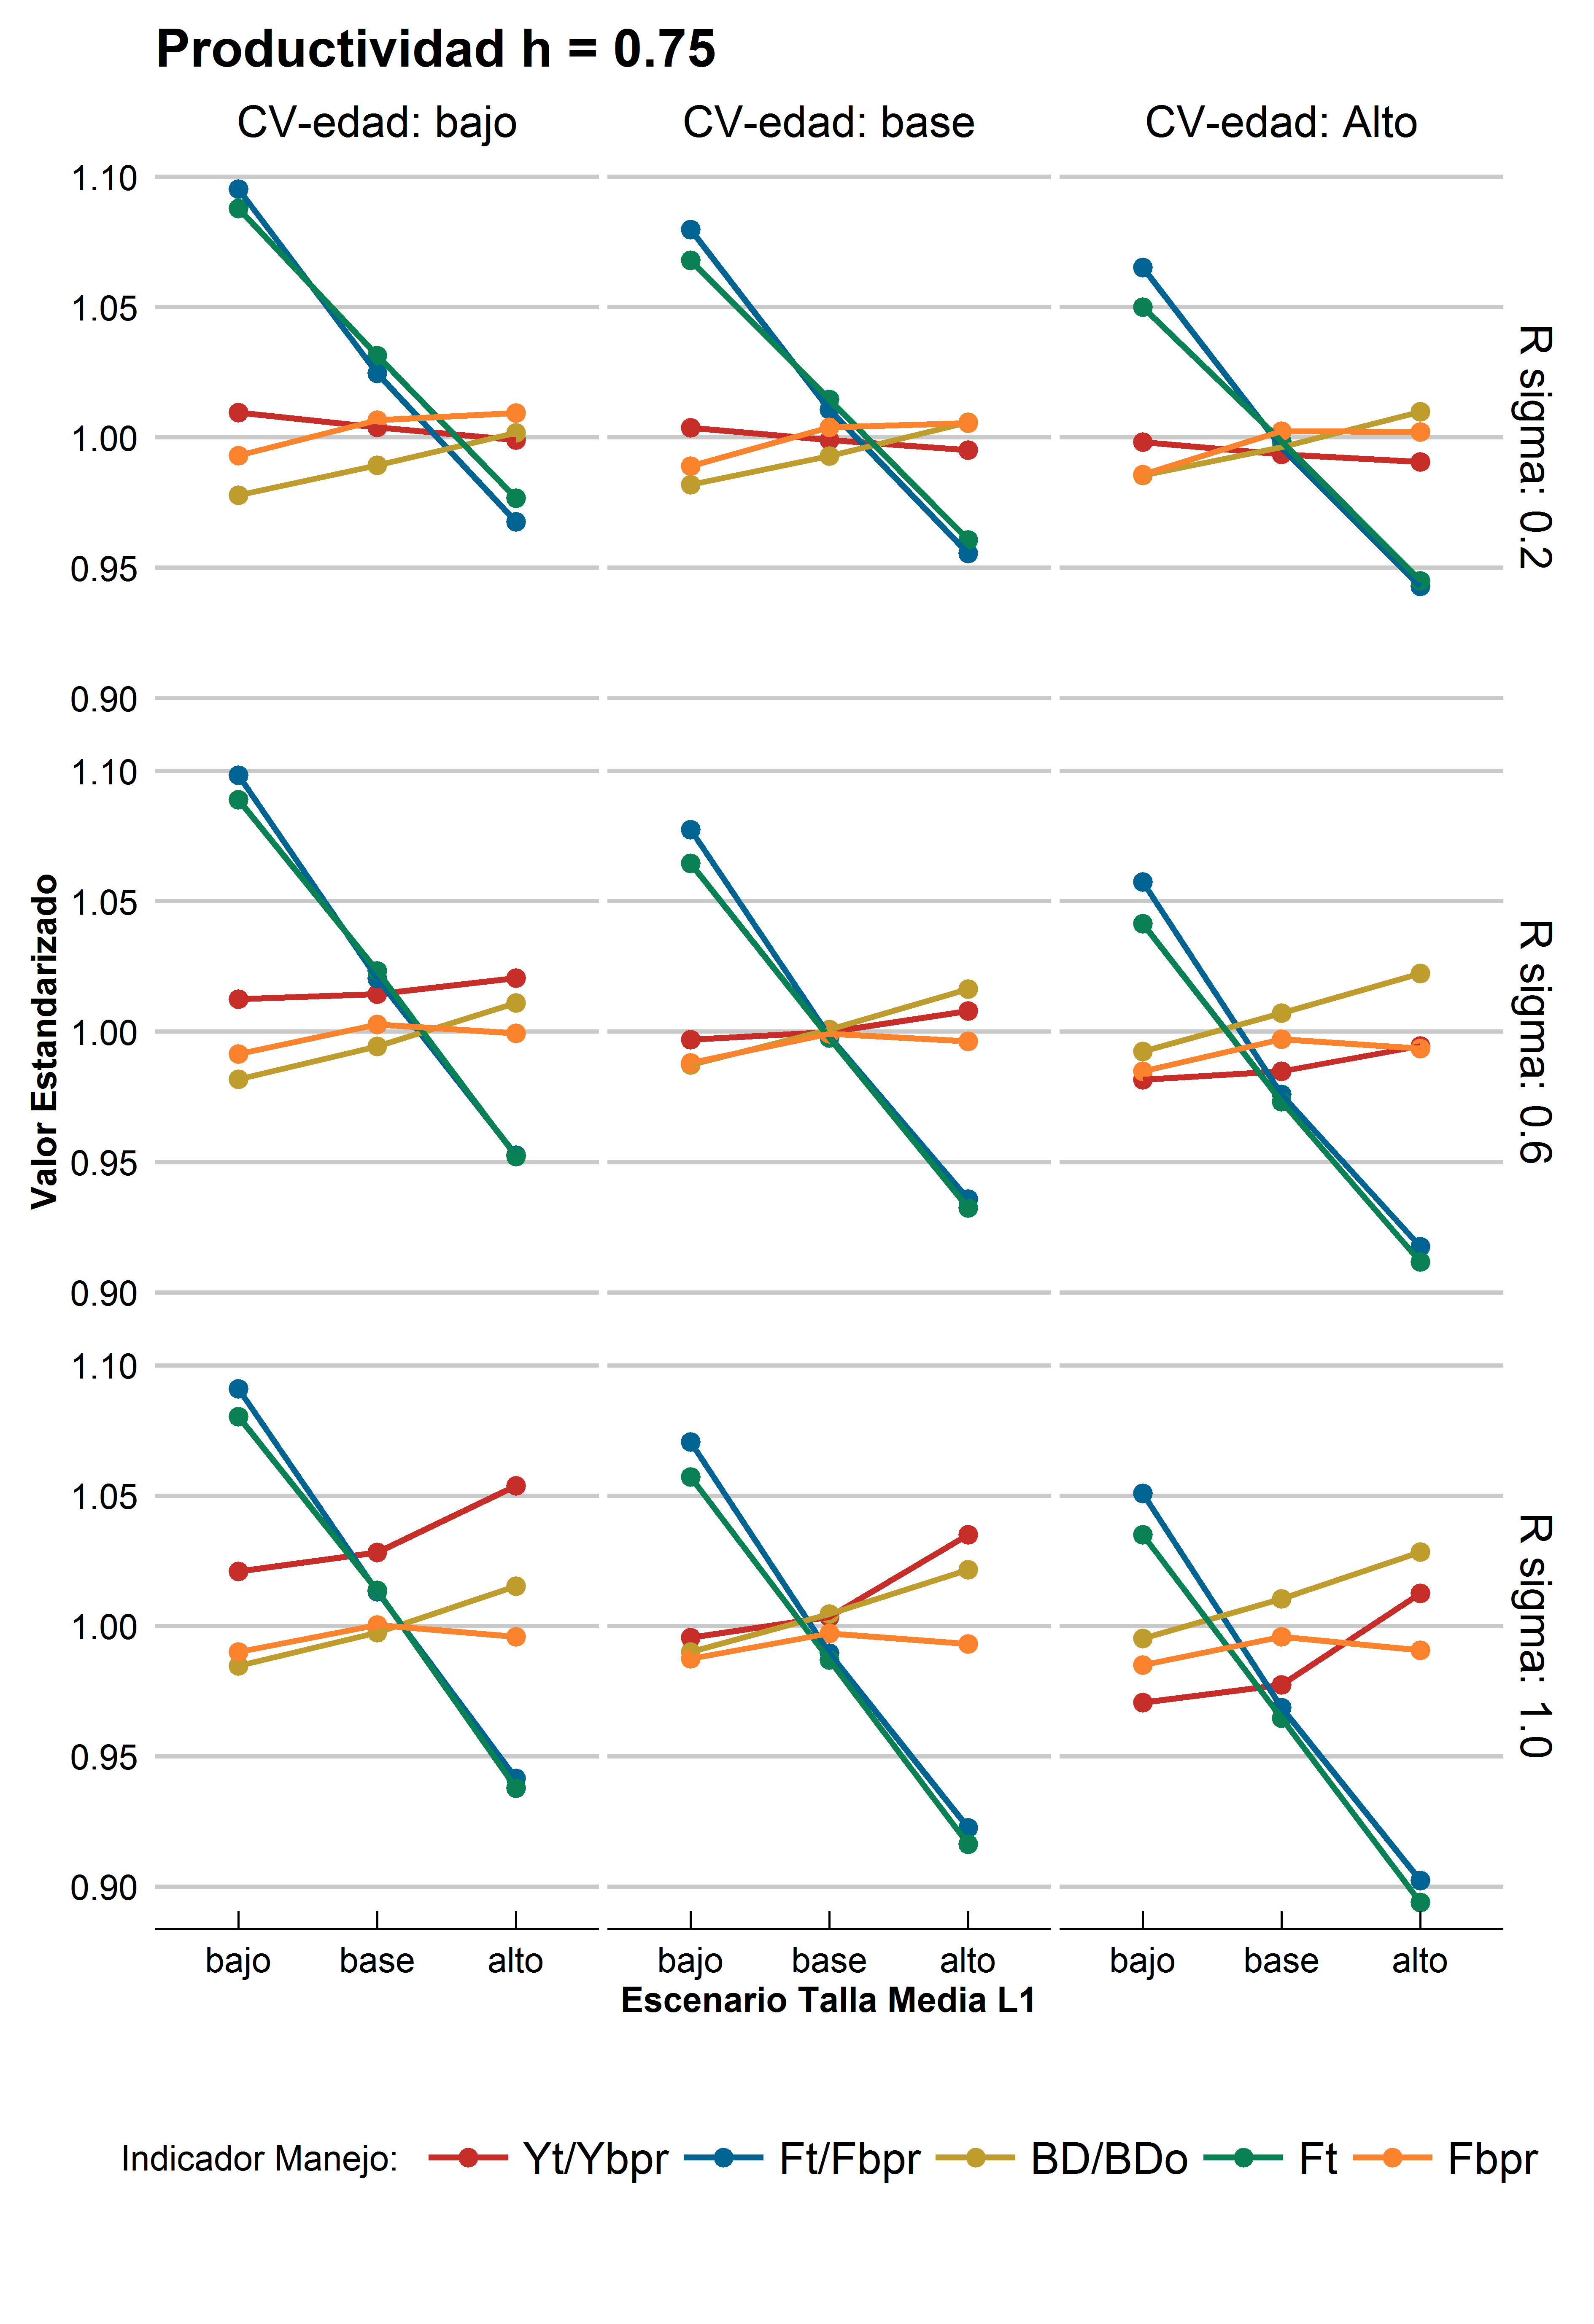
\includegraphics[width=0.70\columnwidth]{figures/steepness-75-var.png}
  \end{center}
\caption{Management advice indicators for scenario with productivity h=0.75. Contained the results of nine (9) scenarios of growth, (x-axis: mean length at-age L1) low (-10\%), Base, high (+10\%). Each column correspond to scenario of VLA, low (-10\%), Base, high (+10\%). Each row correspond to a recruitment variance value.}
\label{figure1}
\end{figure}


\begin{figure}[hbtp]
	\begin{center}
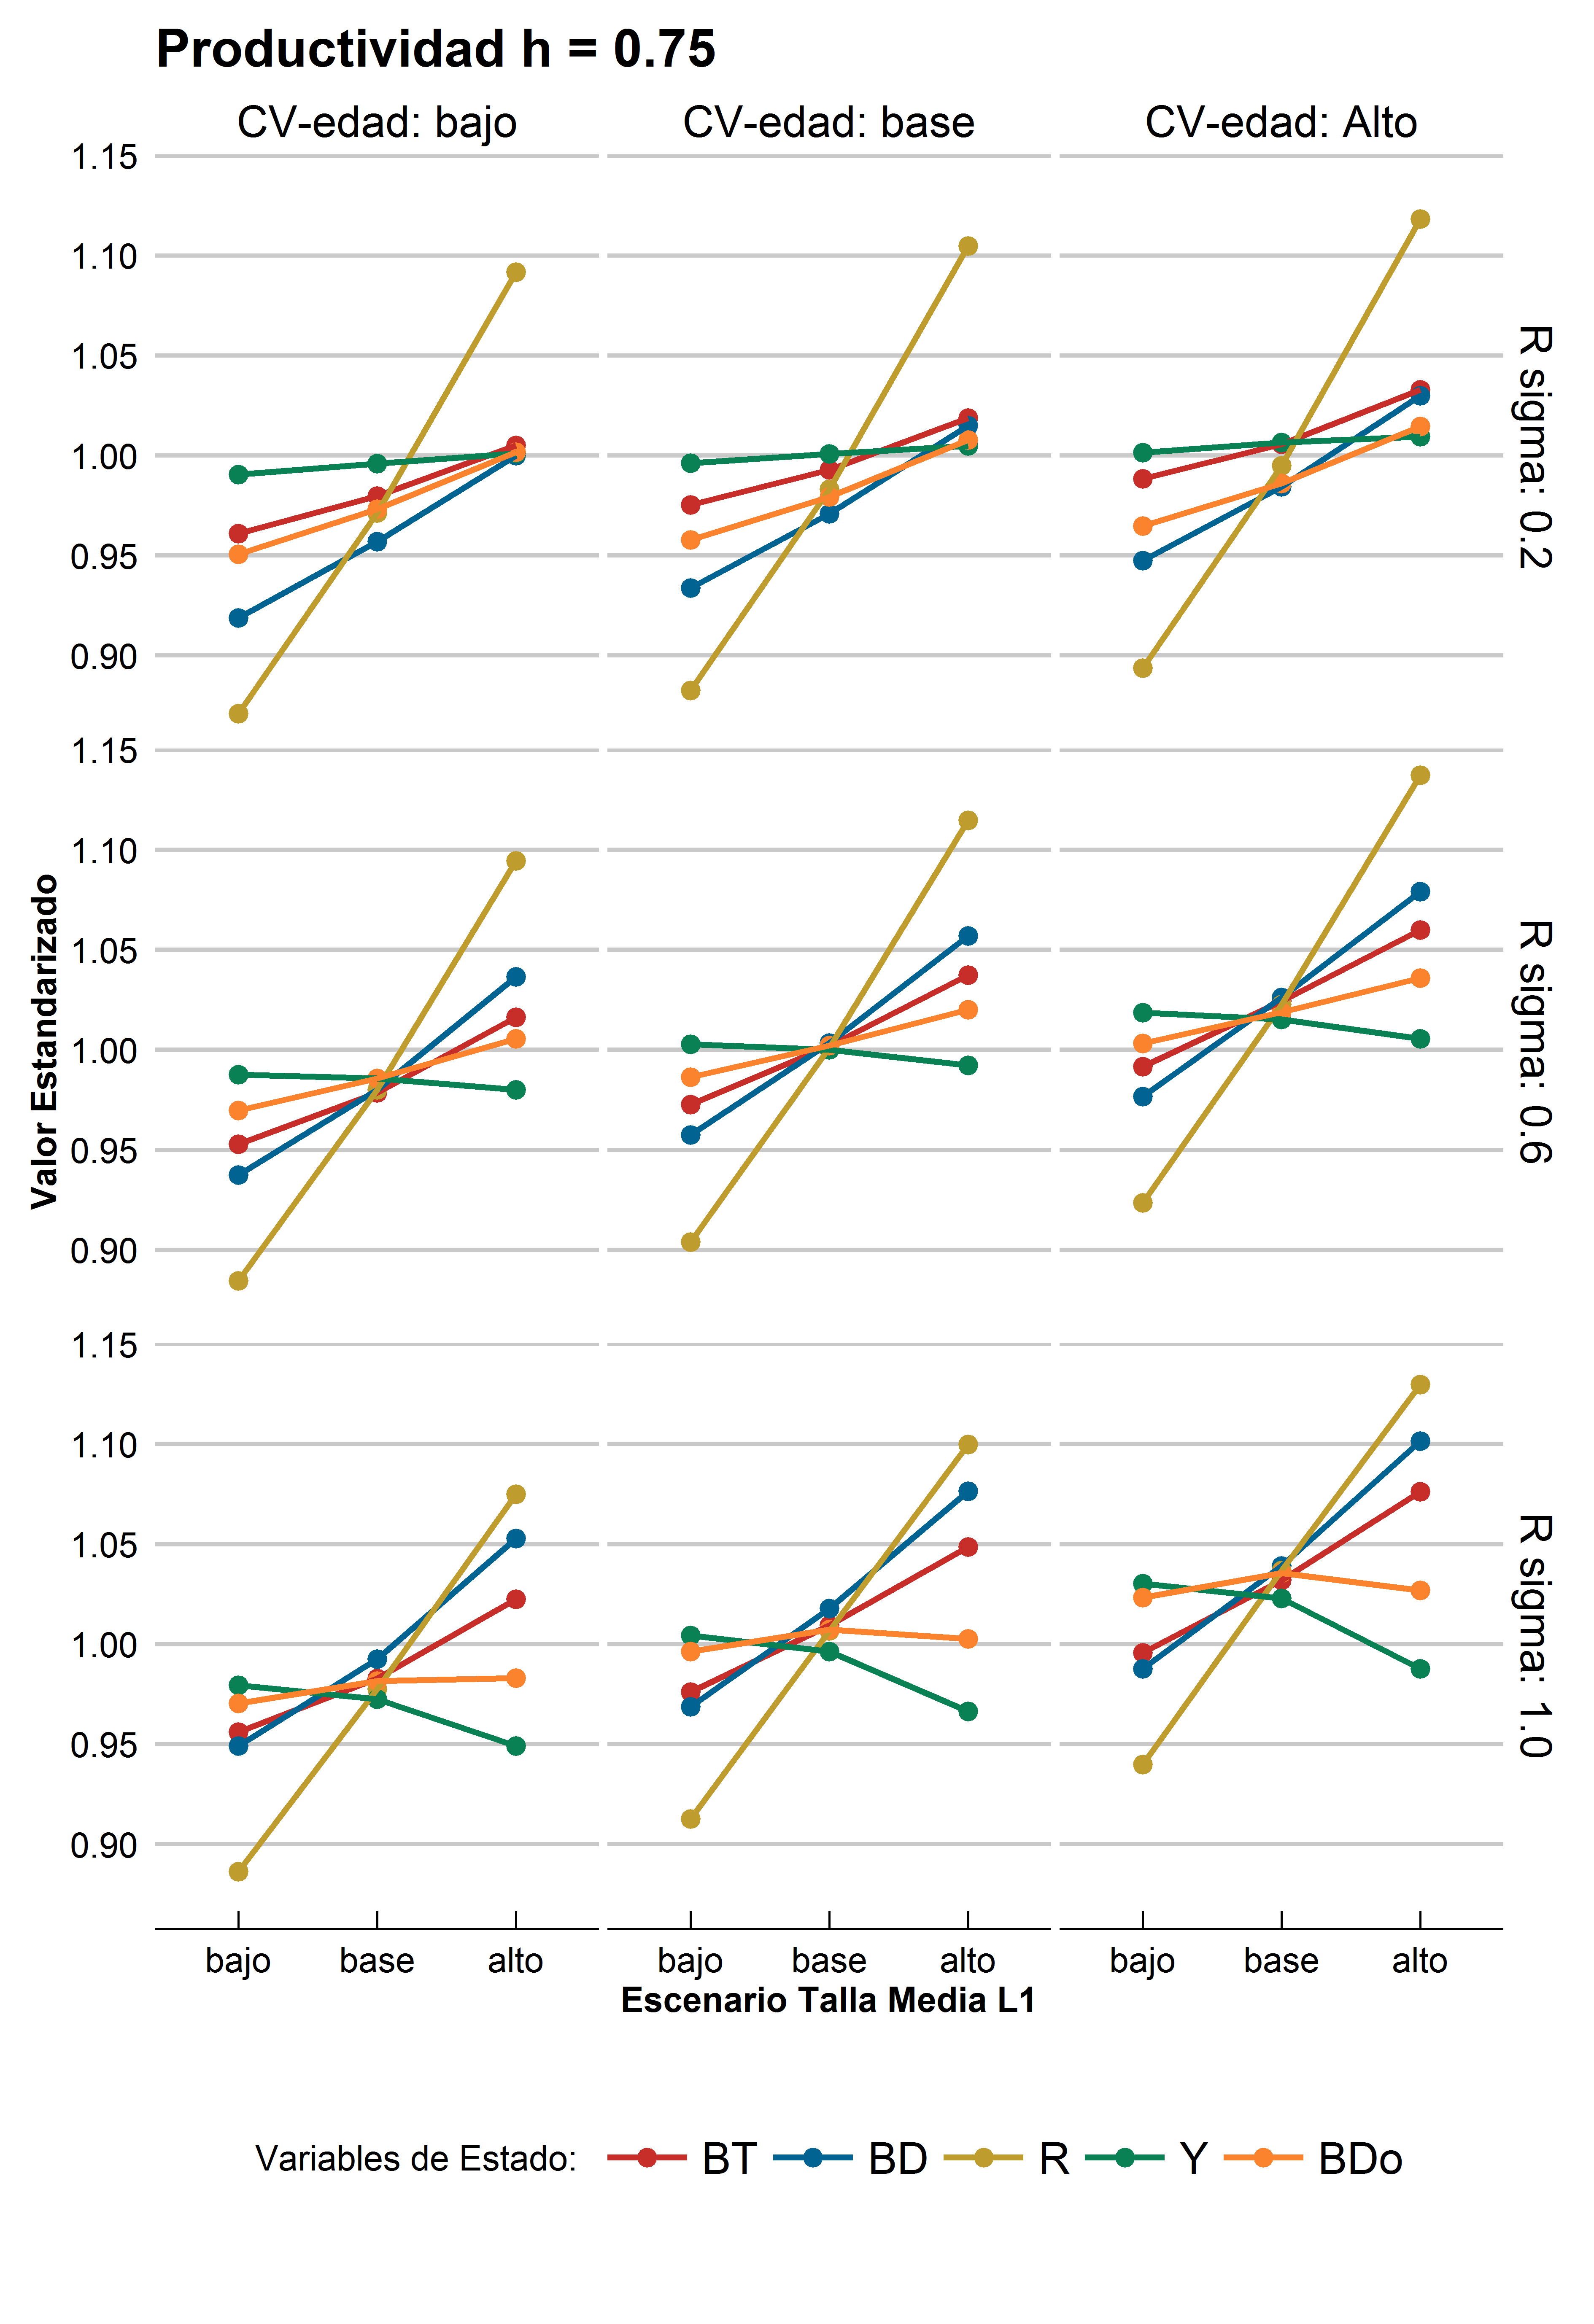
\includegraphics[width=0.70\columnwidth]{figures/steepness-75-estado.png}
  \end{center}
\caption{Stock assessment variables for scenario with productivity h=0.75. Contained the results of nine (9) scenarios of growth, (x-axis: mean length at-age L1) low (-10\%), Base, high (+10\%). Each column correspond to scenario of VLA, low (-10\%), Base, high (+10\%). Each row correspond to a recruitment variance value. Dashed black rectangle indicates the Base Case and should be equal to h=1. TODO---include rectangle}
\label{figure1}
\end{figure}







